
\subsection{One dimensional hydrogen chain}
\label{subsection:1dhydrogen}
We now move to one of the simplest extended \emph{ab-initio} systems, a hydrogen chain in one dimension with periodic boundary conditions. 
We consider the case of $10$ atoms and work in a regime where the inter-atomic distance $r$ is 
relatively large ($r=1.5$ to $3.0$ \AA), such that the system is potentially well described by a one-band Hubbard model 
in terms of primarily $s$-like orbitals, whose form we discuss here. 

For a given $r$, we first obtain single-particle Kohn-Sham orbitals from a set of spin-unrestricted and 
spin-restricted DFT-PBE calculations. The localized orbital basis upon which the RDMs (descriptors) 
are evaluated is obtained by generating intrinsic atomic orbitals (IAO) from the Kohn-Sham orbitals 
orthogonalized using the L\"owdin procedure. These are the orbitals that enter the one-band Hubbard Hamiltonian. 

%\begin{figure}[]
%\centering
%\subfigure[Separation = $1$ \AA]{
%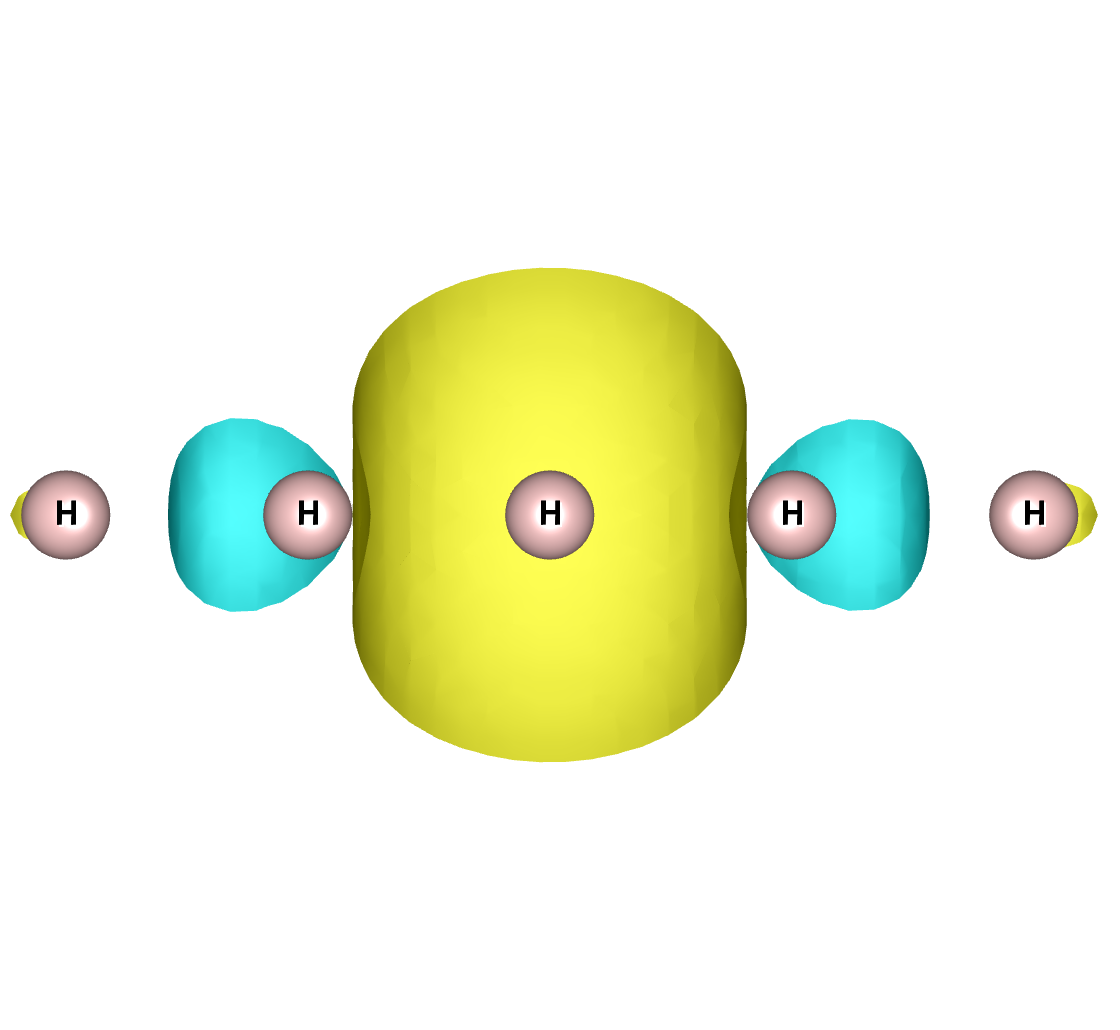
\includegraphics[width=0.20\linewidth]{{./Figures/length1_h_paper_view.orb5}.png}\quad
%}
%\quad
%\subfigure[Separation = $1.5$ \AA]{
%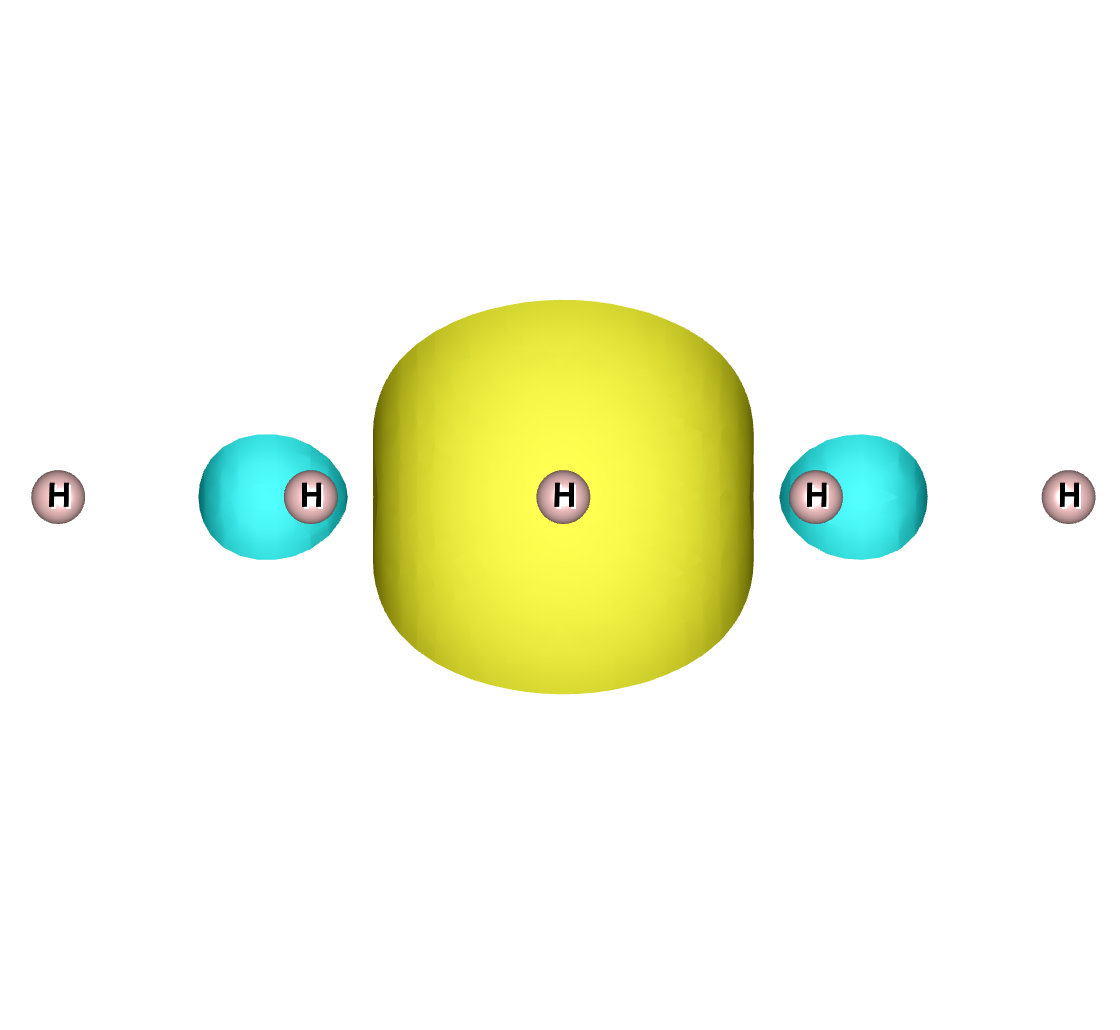
\includegraphics[width=0.25\linewidth]{{./Figures/length1.5_h_paper_view.orb5}.png}%}\quad
%\subfigure[Separation = $2$ \AA]{
%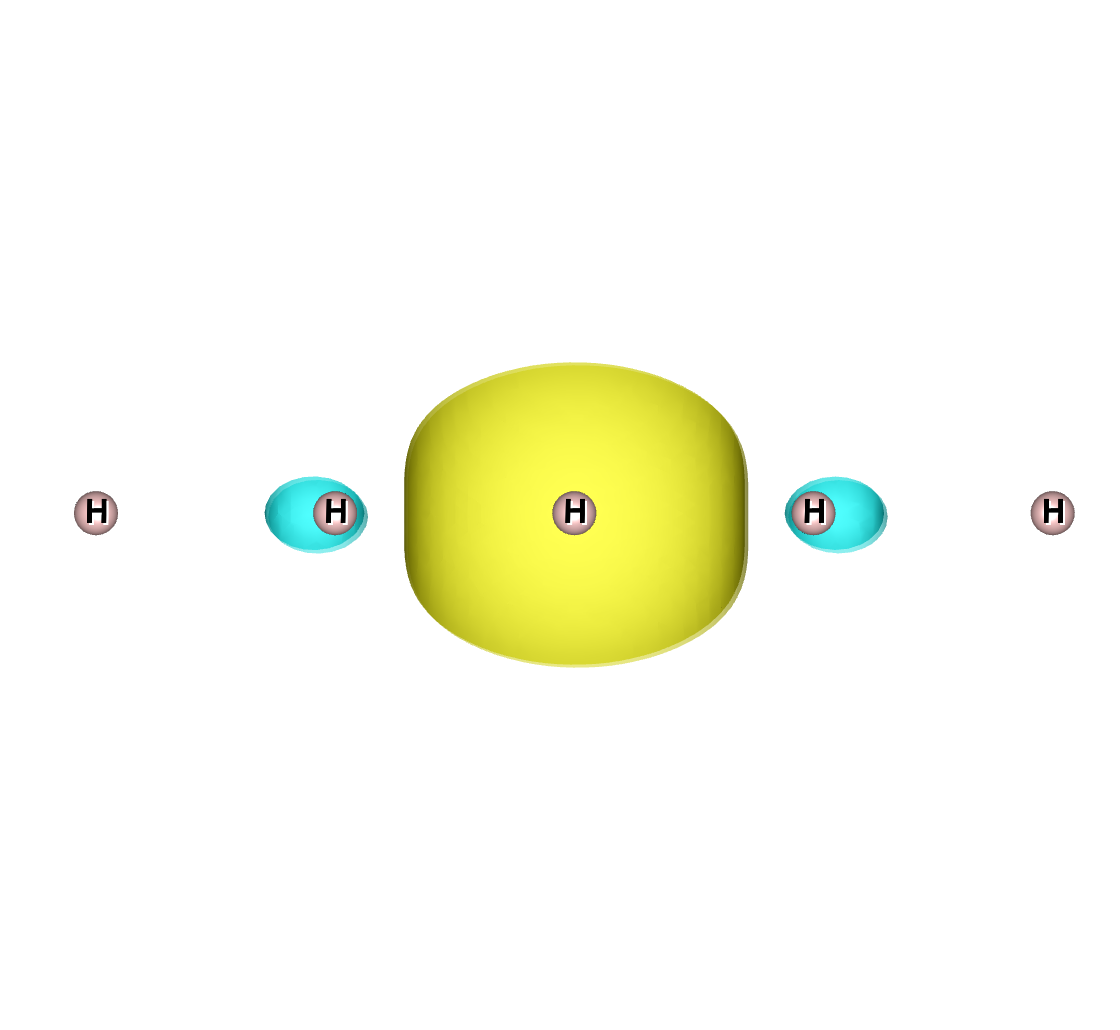
\includegraphics[width=0.20\linewidth]{{./Figures/length2_h_paper_view.orb5}.png}%}
%\caption{Orthogonalized intrinsic atomic orbitals for interatomic hydrogen separation distances equal to $1$, and $2$ \AA \:respectively. }\label{fig:h10orb}%,% $1.5$, and $2$ \AA \:respectively}\label{fig:h10orb}
%\end{figure}

To generate a database of wavefunctions needed for the DMD, we produce a set of Slater-Jastrow 
wavefunctions consisting of singles- and doubles- excitations to the Slater determinant, 
%\HJC{Put Jastrow in front?}
\begin{subequations}
\begin{eqnarray}
| s \rangle = & e^J \Big[a^\dagger_{i \sigma} a_{k \sigma}   | KS \rangle \Big] \,,\\
| d \rangle = & \: e^J \Big[a^\dagger_{i \sigma} a^\dagger_{j \sigma'} a_{k \sigma'} c_{l \sigma}   | KS \rangle\Big] ,
\end{eqnarray}
\end{subequations}
where $|KS\rangle$ is the Slater determinant of occupied Kohn-Sham orbitals, $\sigma$ and $\sigma'$ are spin indices, 
and $a_{i}^\dagger$ ($a_{i}$) is a single-electron creation (destruction) operator corresponding to a particular Kohn-Sham orbital. $e^J$ is a Jastrow factor, optimized by minimizing the variance of the local energy. 
We compute the energies (expectation values of the Hamiltonian) and the RDMs on all the wave functions. 
%Then, having computed the energies (expectation values of the Hamiltonian) and corresponding 
%descriptors for these wavefunctions we verify the independence of the $U$ and $t$ descriptors. 
By computing the trace of the resulting 1-RDMs, we verify that all the electrons present in the system are represented within the localized basis of $s$-like orbitals. If the trace of the 1-RDM falls below the nominal number of electrons for a particular state, this indicates that some higher-energy orbitals are occupied ($p$-like orbitals, in the case of hydrogen), and that the state does not belong to the low-energy manifold. We exclude such states from further analysis. We then fit the one-band Hubbard Hamiltonian using least-squares fitting according to the DMD formalism described in Sec. \ref{sec:theory}.

\begin{figure}
\centering
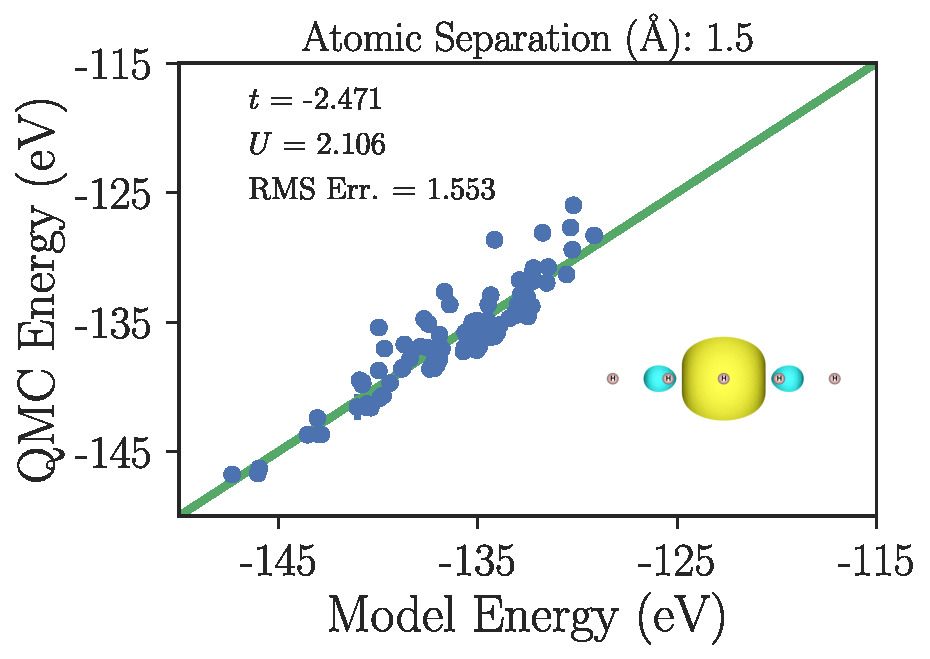
\includegraphics[scale=0.5]{{./Figures/H_chain_fit_model_length1.5_tUs_inset}.pdf}
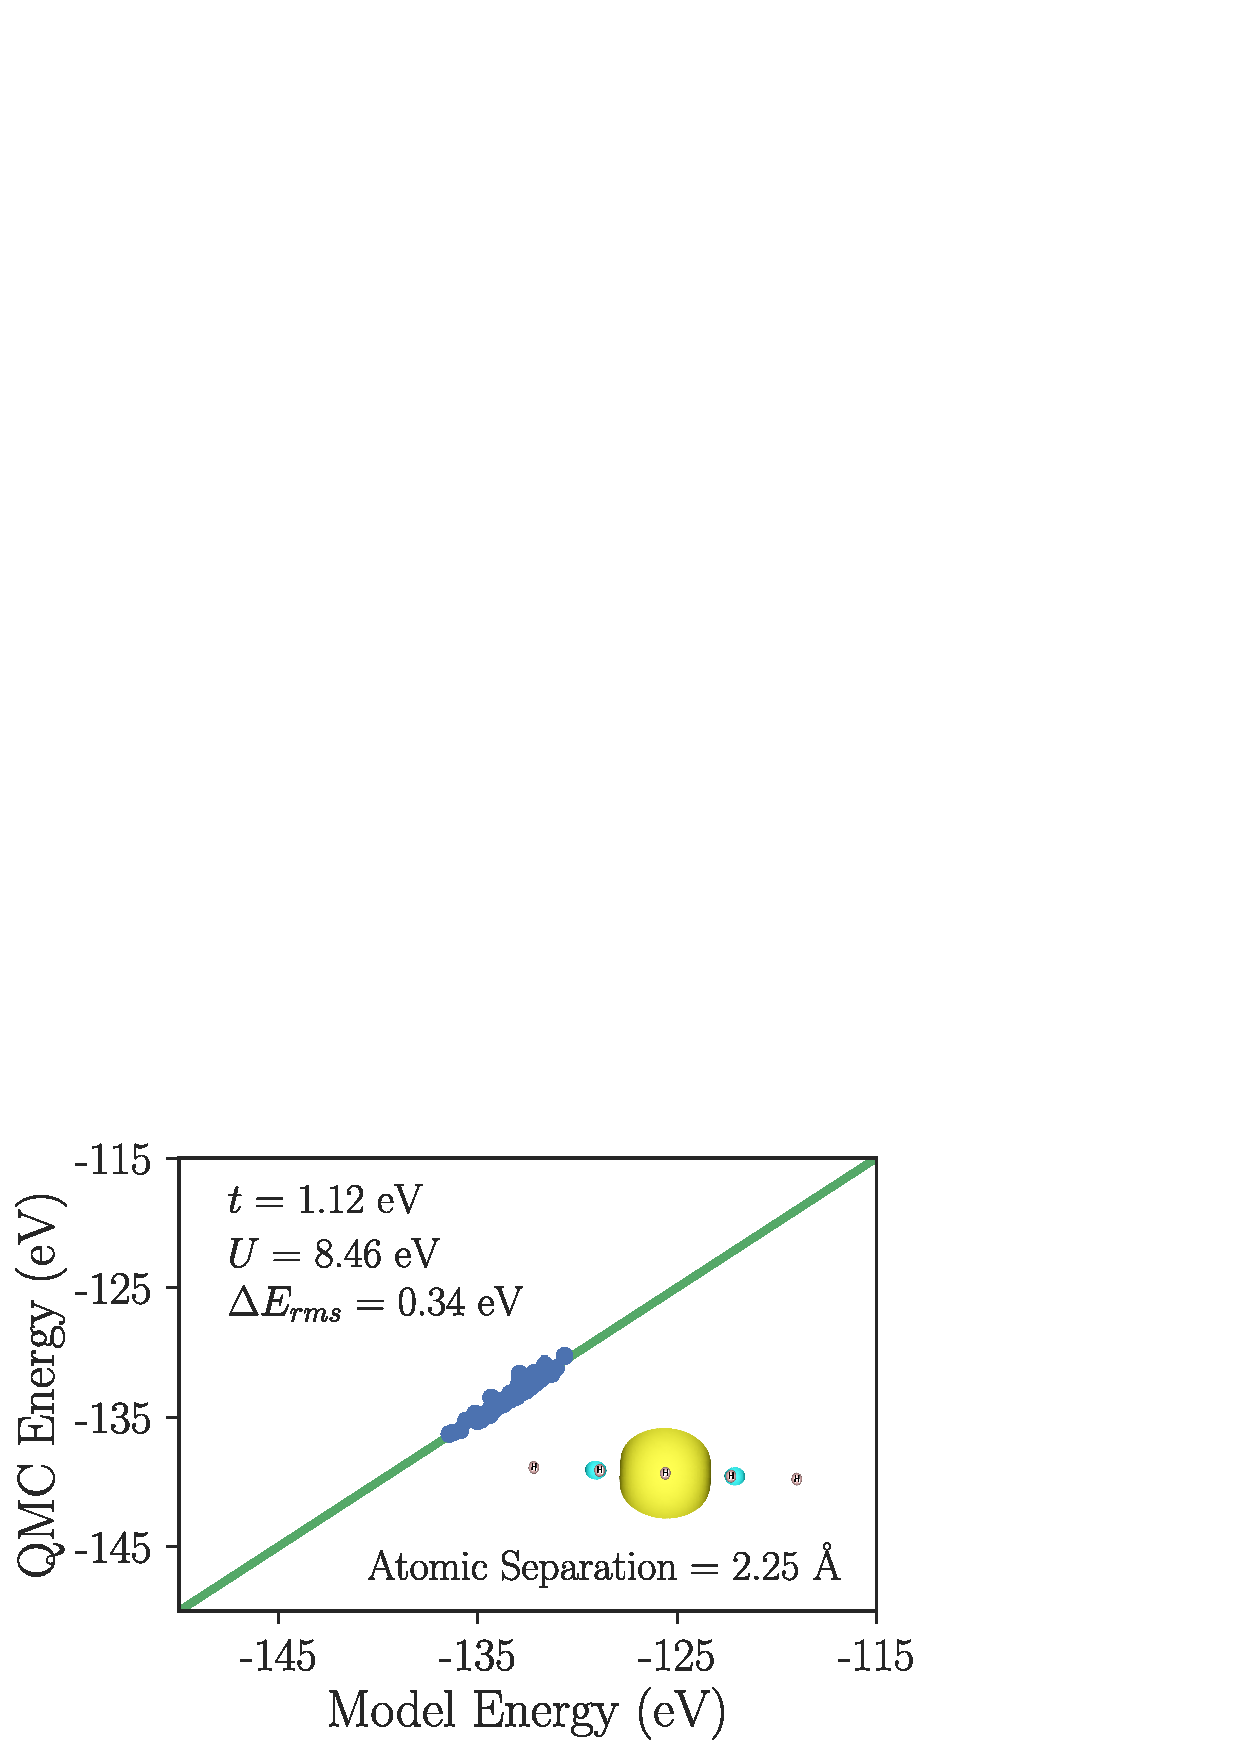
\includegraphics[scale=0.5]{{./Figures/H_chain_fit_model_length2.25_tUs_inset}.pdf}
\caption{DMC energy vs. model energy for the H$_{10}$ chain at 1.5 \AA \:(left) and 2.25 \AA \:(right). Note that the energy range narrows significantly for larger interatomic separation. Insets show intrinsic atomic orbitals upon which we calculated the density matrix descriptors.
}
\label{fig:fit_quality}
\end{figure}

Fig.~\ref{fig:fit_quality} shows our DMD fits for two representative $r$. As expected, the RMS error 
is significantly smaller for larger $r$, verifying the effectiveness of the Hubbard model 
in this limit. The insets show the intrinsic atomic orbitals for which we calculated the density matrix descriptors. Fig.~\ref{fig:Parameters-vs-Bond-t} also shows trends of the fitted value of $t$ 
and $U$ as a function of $r$. Consistent with physical intuition, $t$ decreases towards zero at larger $r$
and the value of $U/t$ rises. 

% Based on these values and the extensive body of work in 1D systems, we expect a Luttinger liquid 
%to insulator transition to occur at $U/t=...$ corresponding to $r=...$.  
The single band Hubbard model does not describe hydrogen chain well at small distance. The one dimensional Hubbard model with $U/t>0$ will always result in an Mott insulating state. However, the metal-to-insulator transition happens at $r_c=\sim1.8$\AA~ for a hydrogen chain \cite{Stella2011}. This indicates that at small distance, the higher energy orbitals play nontrivial roles in stabilizing the metallic state of hydrogen, instead of merely renormalizing the effective strength of U. Meanwhile, at small distance, other interactions term like nearest neighbor Coulomb interaction and Heisenberg exchange interactions also become important at $r<r_c$ \cite{ZhengThesis}. 

\begin{figure}
\centering
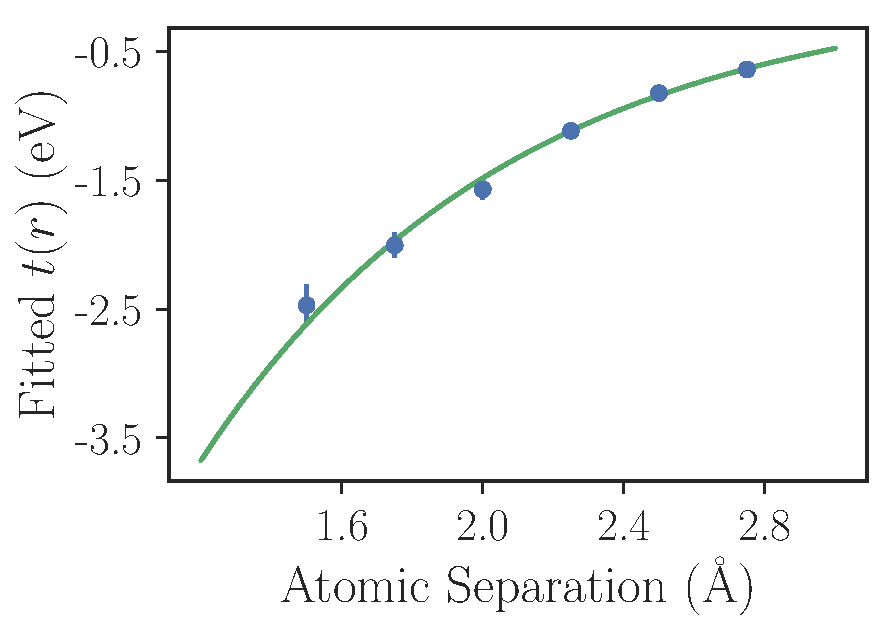
\includegraphics[scale=0.5]{./Figures/fitted_t_values_no_offset_h10_chain.pdf}
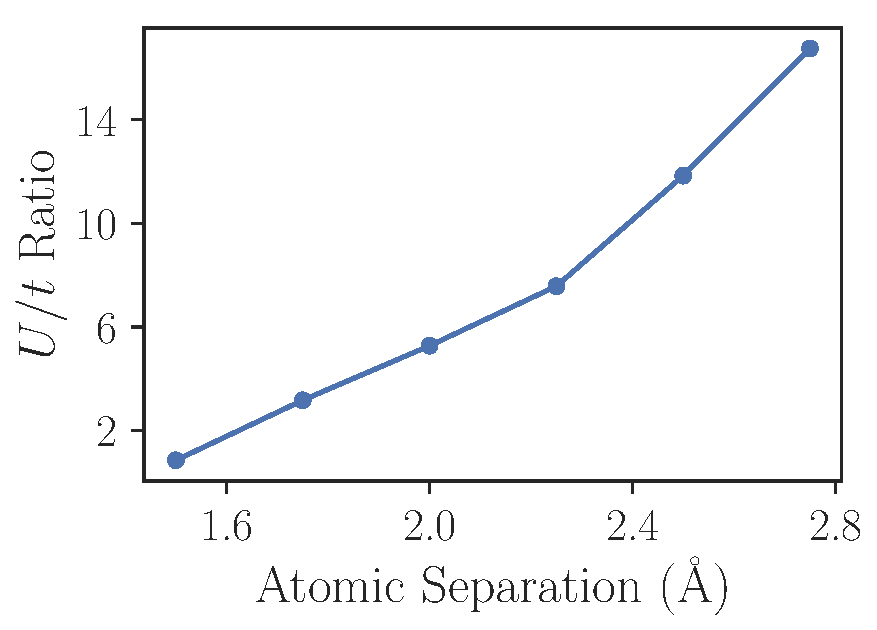
\includegraphics[scale=0.5]{./Figures/Ust_ratio_vs_separation_h_chain.pdf}
\caption{(Left) The one-body hopping $t$ parameter as a function of interatomic distance for the periodic H$_{10}$ chain, obtained from a fitted $U$-$t$ model. $t$ declines to zero as $r$ increases. (Right) The ratio $U/t$ for the fitted parameter values as a function of interatomic separation. The ratio is small at lower bond-lengths, where $t$ is more relevant in describing the system, and larger at longer bond-lengths, where inter-site hopping is less significant. }\label{fig:Parameters-vs-Bond-t}
\end{figure}
